%!TEX root = main.tex

\begin{figure*}[t!]
\centering
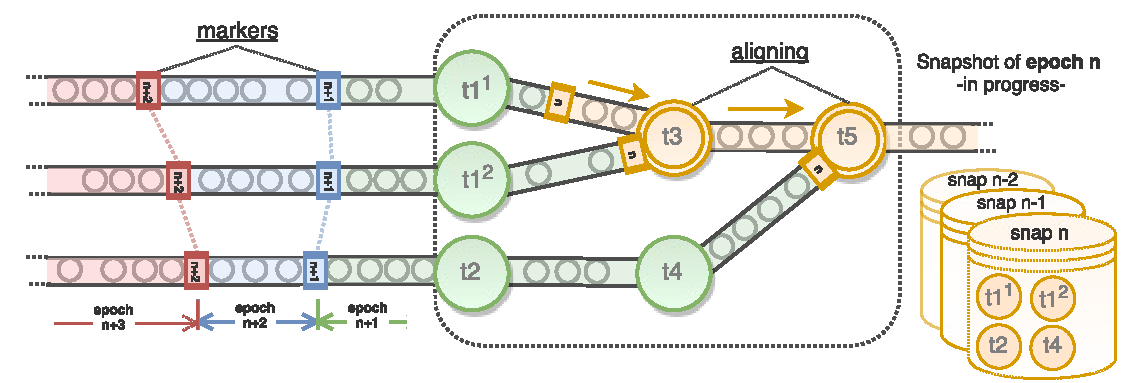
\includegraphics[width=\textwidth]{figures/snapshots-overview.pdf}
\caption{Pipelining Distributed Snapshots on Epochs with Markers.} 
\label{fig:snapshots-overview}
\vspace{-4mm}
\end{figure*}

\section{Core Concepts and Mechanisms}
\label{sec:core}

\subsection{System Model}

Each processing pipeline in Flink translates into a logical directed graph $G = (\mathcal{T}, \mathcal{E})$ consisting of a set of vertices $\mathcal{T}$ representing tasks of finest-grained computation and a set of edges $\mathcal{E}$ reprenting data channels between tasks in $\mathcal{T}$. A task $t \in \mathcal{T}$ can encapsulate the logic of a single user-defined operation (e.g., \texttt{map}, \texttt{filter}, \texttt{fold}) or multiple operations that are fused together. Fusion is a standard logical dataflow optimisation \cite{hirzel2014catalog,chambers2010flumejava} which is also applied on Flink during the composition of $G$. 

\subsubsection{Managed State}

Each stream operation in Flink can declare consistent state and update it continuously in order to keep a summary of the data seen so far. State is a main building block of a pipeline since it encapsulates, at any time the full status of the computation. There are conceptually two scopes upon which managed state operates. For purely data-parallel stream operations such as for example a per-key average, state and associated streams are logically scoped and operate independently for every key. We refer to this state as \texttt{Keyed-State}. For local, per-task computation such as for example a partial machine learning training model, state can be declared in the level of a physical dataflow task, known as \texttt{Operator-State}. Both \texttt{Keyed-State} and \texttt{Operator-State} respectively are transparently partitioned and managed by the runtime of the system. More importantly, the system can guarantee that update operations on managed state will be invoked exactly-once with respect to the input streams. In section \ref{sec:implementation} we explain in detail how the file system facilitates efficient out-of-core state persistence of different state types despite the local  view exposed to the programmer. Below, we briefly explain how managed state can be declared and the basic intuition for each of the state types. \paris{@stefan : Please check and elaborate more in this subsection}

\para{\texttt{Keyed-State}}: Any stream computation can be mapped to a user-defined key space and as a result any associated state will also scoped together with the computation. Typically, data stream records arrive to the system with some domain-specific key such as a user-session identifier, a device address or a geographical location. In the most general case, Flink allows for a user to map any record from its schema domain $\mathcal{S}$ to a given key space $\mathcal{K}$ via the $\texttt{keyby}: \mathcal{S} \rightarrow \mathcal{K}$ operation supported by the \texttt{DataStream} abstract type. Under key scope, state can be allocated dynamically within a user-defined function by using special collections that the model exposes through the API and vary depending on the nature of the state. For append-only state per key (e.g. for storing a pattern sequence or a window) there is a \texttt{ListState} collection supporting an \texttt{add} operation. If  the state is otherwise a value that mutates during the application logic, there is a \texttt{ValueState} type supporting an \texttt{update} operation. Other basic state types such as \texttt{ReduceState} also allow for one or two-step, on-the-fly, distributive function aggregations on managed state. 

\para{\texttt{Operator-State}}: When a DataStream is not scoped by key, state and processing operate per parallel physical instance of a task. This is typical when computation is for example relevant to each physical stream partition such as the source instances of a pipeline that correspond to Kafka consumers in a 1-1 mapping of active offset per partition. Operator-state types are similar to Keyed-State (i.e., \texttt{ListState}, \texttt{ValueState}). 

\subsubsection{State Partitioning and Allocation}

The mapping of a logical dataflow graph to $G$, the physical, distributed execution graph occurs when a pipeline is deployed, on its initial run or upon reconfiguration (e.g., for scale-out). During that stage each logical task $t \in \mathcal{T}$ is mapped to a number of physical tasks $t^1, t^2, \ldots, t^\pi$, each of which gets allocated to available containers throughout a cluster (e.g., using YARN \cite{vavilapalli2013apache}) up to the decided degree of parallelism $\pi \in \mathbb{N^+}$. For tasks that have declared managed state, it is important to consistently allocate data stream partitions or re-allocate in the case of reconfiguration. The partitioning process makes sure that each parallel physical task $t^i , \forall i : 0 \leq i \leq \pi$ will only receive records (and maintain state) that belong to a pre-allocated range of keys. Since the key space $\mathcal{K}$ can be user-defined Flink's runtime pre-partitions keys to an intermediate circular space of ``key-groups'' : $K^* \subset \mathbb{N^+}$ given a maximum parallelism $\pi\text{-max}$ and a hash function $h$ as such:

\noindent $K^* = \{ h(k)\text{ \texttt{mod} }\pi\text{-max}\text{ }|\text{ }k \in \mathcal{K}, \pi\text{-max} \in \mathbb{N^+}, h: \mathcal{K} \rightarrow \mathbb{N^+} \}$

Upon deployment with parallelism $\pi$ key groups are directly allocated per task $t^i$ from $\lceil i \times \frac{\pi\text{-max}}{\pi} \rceil$ to $\lfloor (i+1) \times \frac{\pi\text{-max}}{\pi} \rfloor$. We found that this is a trivial way to pre-partition and reallocate state in a pipeline, typically using a non-cryptographic hash function such as murmur hash. As shown in \autoref{sec:implementation}, state snapshots are materialized and indexed per allocated key group at the backend which allows for trivial reconfiguration. \paris{@stefan I need some input regarding operator state rescaling.}

\subsection{The Pipelined Snapshotting Protocol}

Flink's snapshotting protocol provides a uniform way to capture the complete state of a pipeline and roll it back whenever that is required. We will first explain its intuition followed by a more formal definition of the assumptions and description of the protocol for directed acyclic and cyclic graphs respectively.

\subsubsection{Protocol Intuition}

A continuous stream execution is conceptually divided into logical periods that ``cut'' a distributed data stream into consecutive finite sets of records \ref{fig:abs-general}, which we call \emph{epochs}. An \emph{epoch} can be triggered on-the-fly, periodically by the system or on-demand by the user and is decoupled from any application logic (e.g., windowing constrains). A snapshot of the computation at \emph{epoch} $n$ refers to a copy of the internal state of each task $t \in \mathcal{T}$ after the system fully ingests every input record from the beginning of the computation (\emph{epoch} 0) up to and including \emph{epoch} $n$. In case of a failure during or before a snapshot of \emph{epoch} $n$ is acquired we can simply revert the global state of the distributed dataflow graph to a previous \emph{epoch} (e.g., $n-1$). A discrete approach to snapshotting would be to let the distributed dataflow fully ingest \emph{epoch} $n$ independently, store the internal state of each task $t \in \mathcal{T}$ and proceed with \emph{epoch} $n+1$ (similarly to micro-batching \cite{zaharia2012discretized}). However, this approach generally leads to high latency and underutilization costs related to the coordination of a discrete execution which cannot be amortized trivially \cite{venkataramandrizzle}. Furthermore, other protocols either disrupt normal execution \cite{murray2013naiad,jacques2016consistent} or are incapable of supporting weakly connected graphs \cite{chandy1985distributed} which are the norm in distributed dataflow processing.

Instead, Flink's snapshotting protocol pipelines progressively the partial acquisition of task states to eventually acquire a complete snapshot, respecting \emph{epochs}, while running concurrently alongside normal operation. Special markers are injected in each data stream partition at the dataflow sources, coordinated by the runtime and get disseminated throughout the dataflow graph as depicted in \autoref{fig:snapshots-overview}. Markers signal distributed tasks of new epochs and thus aid to establish the appropriate moment to snapshot each local state and proceed with further processing promptly. Tasks with multiple inputs execute an \emph{alignment} phase (e.g., tasks $t3$ and $t5$ in \autoref{fig:snapshots-overview}) upon which they prioritize inputs from pending \emph{epochs}. Alignment is decentralized and eliminates the need to forcefully consume an epoch or log records in transit in the case of acyclic graphs. As we explain in more detail further, cyclic graphs require partial channel logging only limited to each dataflow cycle. The snapshotting protocol is coordinated centrally by the \emph{JobManager} and each invocation eventually completes or gets aborted (e.g., when a failure occurs). In either case the overall dataflow computation can always progress without interruptions and consecutive snapshots will eventually complete.

\subsubsection{Main Assumptions}

The protocol assumes a fail-recovery, deterministic process model \cite{elnozahy2002survey} where a partial process failure can be masked by redeployment and restoration of prior operational states. In detail, our protocol builds on the following assumptions:
\TODOX{revisit this part}

\begin{itemize}
	\item Input data streams are durably logged and indexed by an external logging system such as Apache Kafka \cite{kreps2011kafka}. That means that dataflow sources can trivially re-consume input from a specific logical time by requesting an offset per stream partition. 
	\item Directional data channels between tasks are quasi-reliable, respect a FIFO delivery order and can be blocked or unblocked. When a channel is blocked in-transit messages are internally buffered (and possibly spilled to disk) and can be delivered on that end once it unblocks.
	\item Tasks can trigger blocking or unblocking operations on their input data channels and send messages through their output channels. Broadcasting on output channels is also supported.
\end{itemize}

\subsubsection{Directed Acyclic Graphs}

\subsubsection{Dealing with Cycles}

\subsection{Savepoints and Rollback}

\paris{Savepoints and Checkpoints are now the same thing but we can probably highlight here how we can not only reconfigure parallelism but also push patches and use this for pipeline versioning}

\paris{Recovery is probably the weakest part of state management. We restart the whole thing whenever we have to reconfigure and this is honestly a bit bad but hey it's simple. (also spark does this for every microbatch so maybe it is not that sad)}